\section{Software}

\subsection{... CODA DAQ software ... (Abbott)}

CLAS12 DAQ system is based on CODA (Fig.~\ref{fig:coda_diagram}), short for CEBAF Online Data Acquisition. It is a kit of parts that allows the researcher to implement a data acquisition system. The scale of the system can range from a few detector channels in a test stand to tens of thousands of channels in a large detector installation in one of the halls. CODA achieves this scaling through modularity and provides a set of hardware components along with complementary software components.

\begin{figure}[hbt]
	\centering
	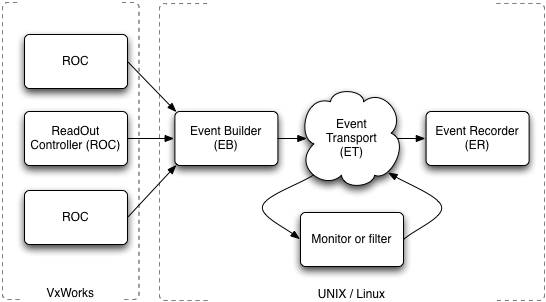
\includegraphics[width=1.0\columnwidth,keepaspectratio]{img/coda_diagram.png}
	\caption{CODA System Diagram}
	\label{fig:coda_diagram}
\end{figure}


\subsection {Runcontrol(Sergey)}

The CODA DAQ system includes a run control facility consisting of a back-end run control supervisor and a front-end graphical operator display that connects to the supervisor and controls its operation. The supervisor in turn controls operation of the many CODA components that participate in the run. The latter are defined in run configuration files that the operator chooses at startup. The gui presents the operator with a choice of possible actions that depend on the current state of the run. The supervisor translates the operator choice into appropriate commands to the individual components. Alternatively, limited communication with the supervisor can be performed via command-line scripts.
The supervisor in addition monitors the health and operation of the CODA components and warns the operator or pauses the run if problems are detected.


\subsection{Front End Libraries(Moffit)}

\subsection{Frontend Libraries}

Just an outline ATM

GEFANUC driver:
\begin{itemize}
\item Customized Kernel Driver and Userspace Interface
\item C API provides:
   \begin{itemize}
   \item Setup of VME inbound and outbound windows
      \begin{itemize}
      \item Permanent windows: CRCSR, A16, A24, A32
      \item Map of these windows into userspace
      \end{itemize}
   \item Allocate of Physical Memory for DMA
      \begin{itemize}
      \item Map of this memory into userspace
      \end{itemize}
   \end{itemize}
\end{itemize}

JVME Userspace Driver:
\begin{itemize}
\item C API provides
  \begin{itemize}
  \item common userspace interface to GEFANUC driver and others.
  \item Initialization of kernel driver and default VME windows
  \item Maps VME bridge registers into userspace
    \begin{itemize}
    \item Provides userspace configuration and operation of DMA
    \end{itemize}
  \item Initialization of and access to shared memory mutex for intra-process cooperation during DMA
  \end{itemize}
\end{itemize}

Frontend Libraries
\begin{itemize}
\item C APIs provide
  \begin{itemize}
  \item module register mapping in VME windows to memory structures.
  \item configures modules for readout via
    \begin{itemize}
    \item programmed i/o
    \item Single module DMA
    \item Multiple module DMA
       \begin{itemize}
       \item Token passing (P0/VXS and CBLT) with common A32 address range
       \item Linked List DMA
       \end{itemize}
    \end{itemize}
  \end{itemize}
\end{itemize}



\subsection{Readout Controller(Abbott)}

Readout Controller (ROC) software component is the program running on front-end controllers such as Intel-based VME/VXS crate controllers, VTP trigger boards or regular Linux servers - any hardware receiving data from front-end electronics. On the startup ROC starts three threads, after that it jst controlls thread health and communicates with run control process. Three threads (readout, process and network) build a chin passing data from one to another communicating over circular buffers.

First (readout) thread receives data from front-end electronics and places them into first circular buffer. That thread can run in pooling mode occupying entire cpu core, or in interrupt mode. CLAS12 are using mostly pooling mode which has adequate performance on multi-core controllers.

Second (process) thread reads data from first circular buffer and perform needed data processing, in particular it does so-called disentangling and data sanity check. Results placed into second circular buffer. That component can create its own threads to burst processing power.

Third (network) thread reads data from second circular buffer and send it over network to the Event Builder.

First and second threads have user part which compiled separately and downloaded dynamically, it allows users to develop experiment-depemdent code without touching CODA framework.



\subsection{Event Builder (Graham)}

Event Builder is the program receiving data from all readout controllers and glueing it into events. Building process is based on event number, event type and timestamp of the data fragments: for every particular event all three values have to be identical for all data from all readout controllers. In case of any difference DAQ will be stopped and error reported.

Event Builder consists of receiving and building parts. Receiving part contains set of independent threads, one per readout controller connected to it by TCP protocol. Every thread receives data and place it into internal buffer. If buffer becomed full thread stops receiving data, effectively propagating busy condition back to readout controller.
Building part has the number of identical building threads, which takes turns by getting data from receiving part internal buffers, building events and placing them into Event Transfer system.

Total number of Event Builder threads in CLAS12 DAQ exceeds hundred, so the number of network connections from readout controllers. Because of that it have to run on powerful server, usually the one with many cpu cores, big memory and high bandwidth network card. CLAS12 is using DELL R730 server with 32 cores, 64GByte memory and 40Gbit network card. That server is adequate for CLAS12 DAQ requirements.


\subsection{Event Transfer (Carl)}

Event Transfer (ET) system allows multiple connections to the data stream, needed for online data monitoring and possibly data or/and event reduction. It consists of ring of buffers, one per event, filled by Event Builder and accessed by one or several processing programs. Every processing program can request to see every event or subset of events based on selecting algorithm. There is a possibility to access ET system remotely, as well as create a chain of ET systems running on different servers effectively increasing processing power. Last program attached to ET system usually Event Recorder.

\subsection{Event Recorder (Sergey)}

Event Recorder (ER) is the program receiving data from ET system and recording data files into the disk. It can write data in one or several files in parallel (so-called multi-stream mode). If multi-stream mode is used event order is preserved, but it requires the allocated memory size to be bigger then the number of streams multiplied by the file size.


\subsection{Messaging System (ActiveMQ) (Sergey)}

Messaging system in CLAS12 DAQ is based on ActiveMQ library and its C++ extension. Two ActiveMQ servers used to route all communiations. The number of connections to ActiveMQ is several hundreds, and the number of messages sent every second is several tens of thousands, with data volume few tens of Megabytes per second. Messaging system is used in particular to monitor and control DAQ components, in addition to the Runcontrol.


\subsection{Runtime Database (RCDB) (Sergey)}

JLAB-designed mysql-based Runtime Database (RCDB) is used to store run parameters and statistic. It has web interface (Fig.) and provides interface to various languages including C++ and Java.


\subsection{Online Data Monitoring (Raffaella,Cole)}

CLAS12 Online data monitoring is the set of programs attached to Event Transfer System and processing data in real time. One of such program's output is shown on Fig.



\subsection{CSS for DAQ, communication with DAQ (Nathan)}



\subsection{ROOT for DAQ (FT) (Andrea)}

A ROOT-based system was developed to display integrated quantities from the CLAS Trigger system in the form of 1D
and 2D histograms. The system is made by three different applications: a histogram sender running on each VTP, a
histogram receiver running on a DAQ server, and a user-configurable GUI client. Each histogram sender application
defines a set of 1D and 2D histograms to report trigger data specific to the CLAS12 subsystem handled by the VTP it is
running on. Histograms are refreshed at a fixed rate and streamed to the DAQ server in the form of JavaScript Object
Notation (JSON) messages, exploiting the previously described ActiveMQ infrastructure. Each message contains: the
histogram name, the number of bins, and a data array with the number of counts in each bin. The message receiver
application is responsible for decoding these messages, and of creating ROOT histograms from them. Finally, the client
application displays ROOT histograms to the user through a customizable GUI.

The GUI is composed of a programmable number of independent frames, with different histograms in each of them.
Typically, each frame contains histograms related to the same CLAS12 subsystem. The GUI structure is specified through
a configuration file passed as a command-line option when running the client. Communication between the message
receiver/ROOT histogram produced application and the user client is handled through the ROOT TSocket mechanism.
Figure~\ref{fig:plot_andrea} shows a GUI reporting histograms from the Forward Tagger system~\cite{ft-ref}: two
2D histograms showing the distribution of electromagnetic cluster hits in the Forward Tagger Calorimeter, and two
1D histograms showing the electromagnetic cluster energy distribution. The right (left) column reports histograms for
electromagnetic clusters  with (without) a matching hit in the Forward Tagger Hodoscope.

\begin{figure}[t]
	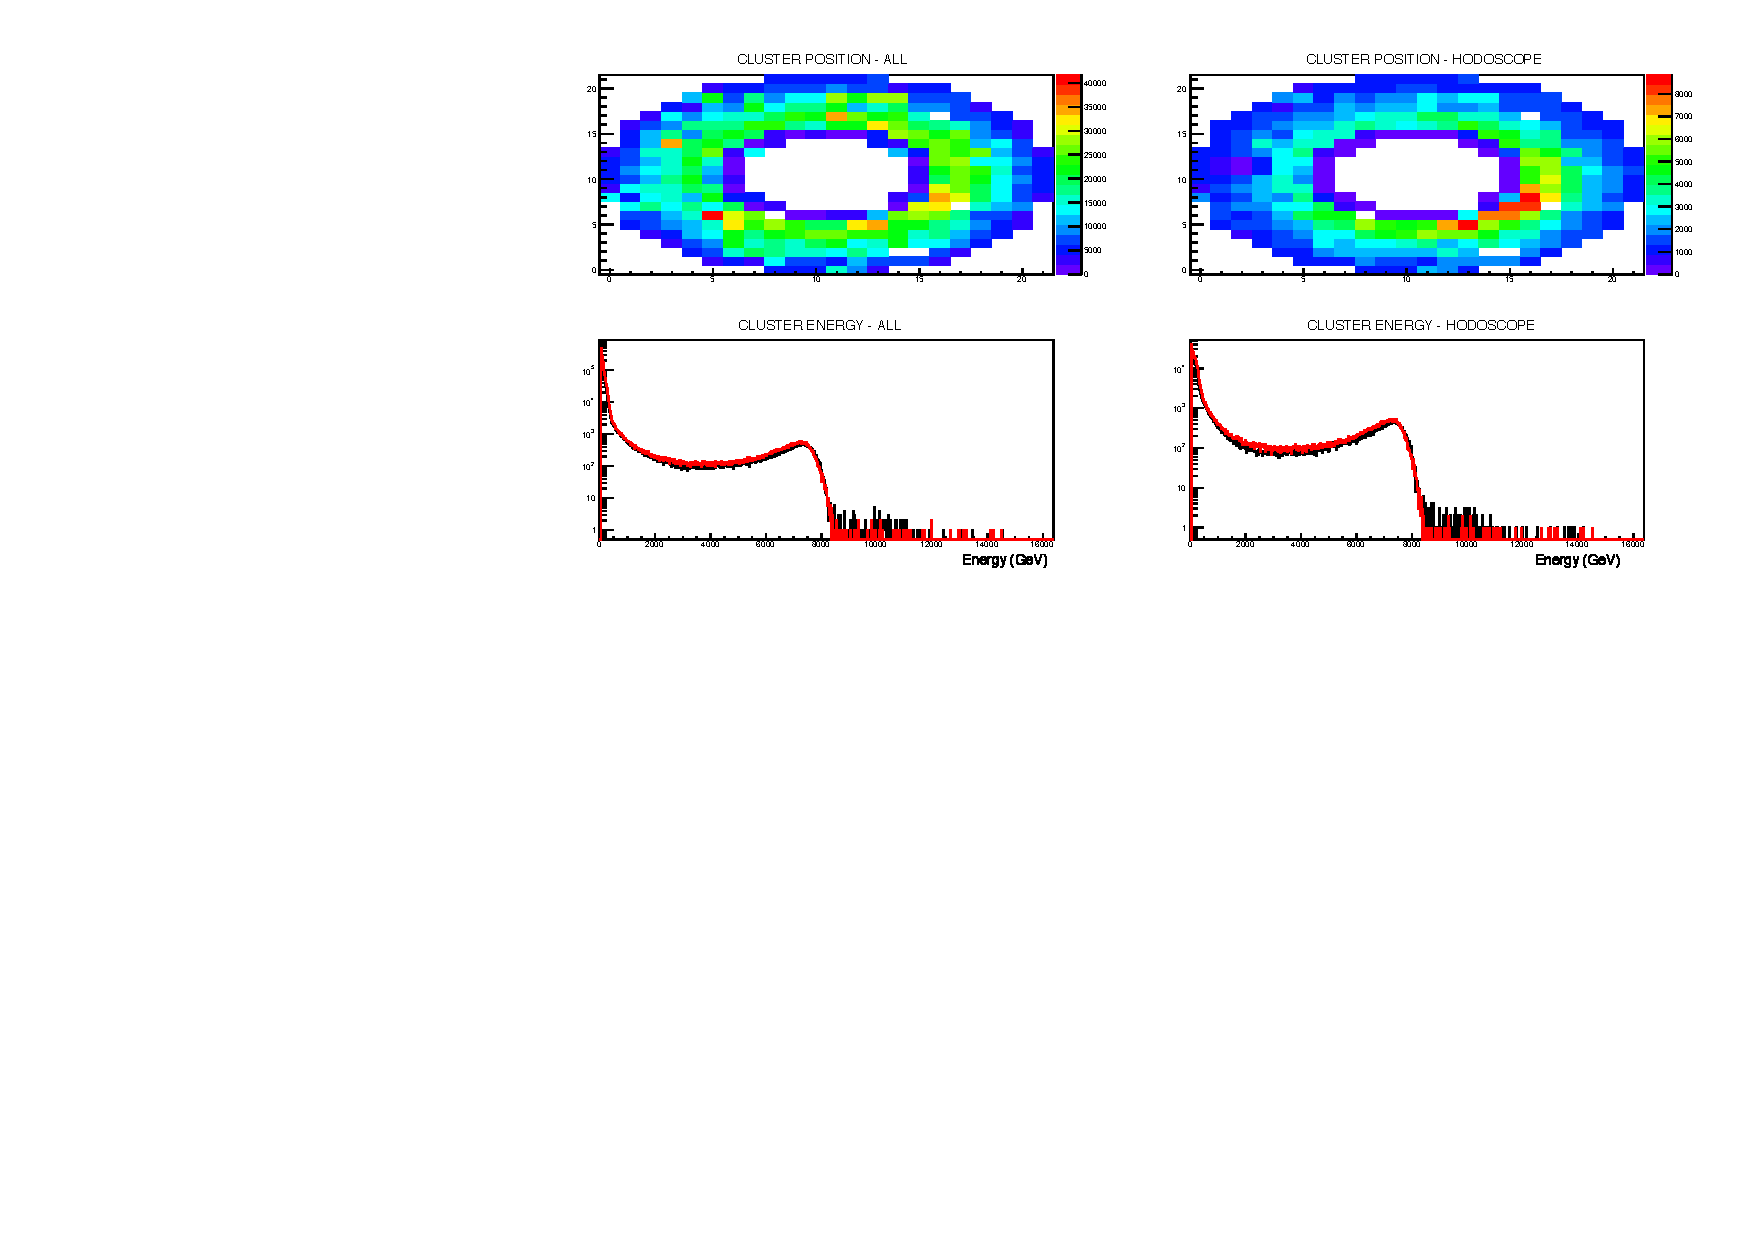
\includegraphics[width=1.0\columnwidth]{img/plotAndrea.pdf}
	\caption{Example of a ROOT-based GUI to monitor trigger data for the specific case of the Forward Tagger
        detector~\cite{ft-ref}. The top histograms report the distribution of electromagnetic cluster hit positions, while
        the bottom histograms report the electromagnetic cluster energy distribution. The right (left) column reports
        histograms for electromagnetic clusters  with (without) a matching hit in the Forward Tagger Hodoscope.}
	\label{fig:plot_andrea}
\end{figure}



\subsection{CLAS Event Display (Heddle)}

The CLAS12 event display (ced) is a full-function graphical application that displays on-line (and off-line) events using various representations of CLAS12 called views. The views are independent windows that the user can pan, zoom, scroll, etc. Some of the views are geometrically faithful, and some are designed for maximal information content as opposed to realism. The primary purpose and utility of ced, when used on-line as part of the DAQ system, is for additional monitoring. While running, ced will display an event from the live stream at a selectable rate, typically one every two seconds. A quick glance at ced will confirm, for example, that there are data in the drift chambers that appear to form tracks. In this way it serves as an early warning of problems with detectors and/or the data stream. It is also possible to operate ced in a mode where it creates graphical histograms or occupancy overlays. A typical view from ced is shown in Fig.~\ref{fig:ced}.

\begin{figure}[hbt]
	\centering
	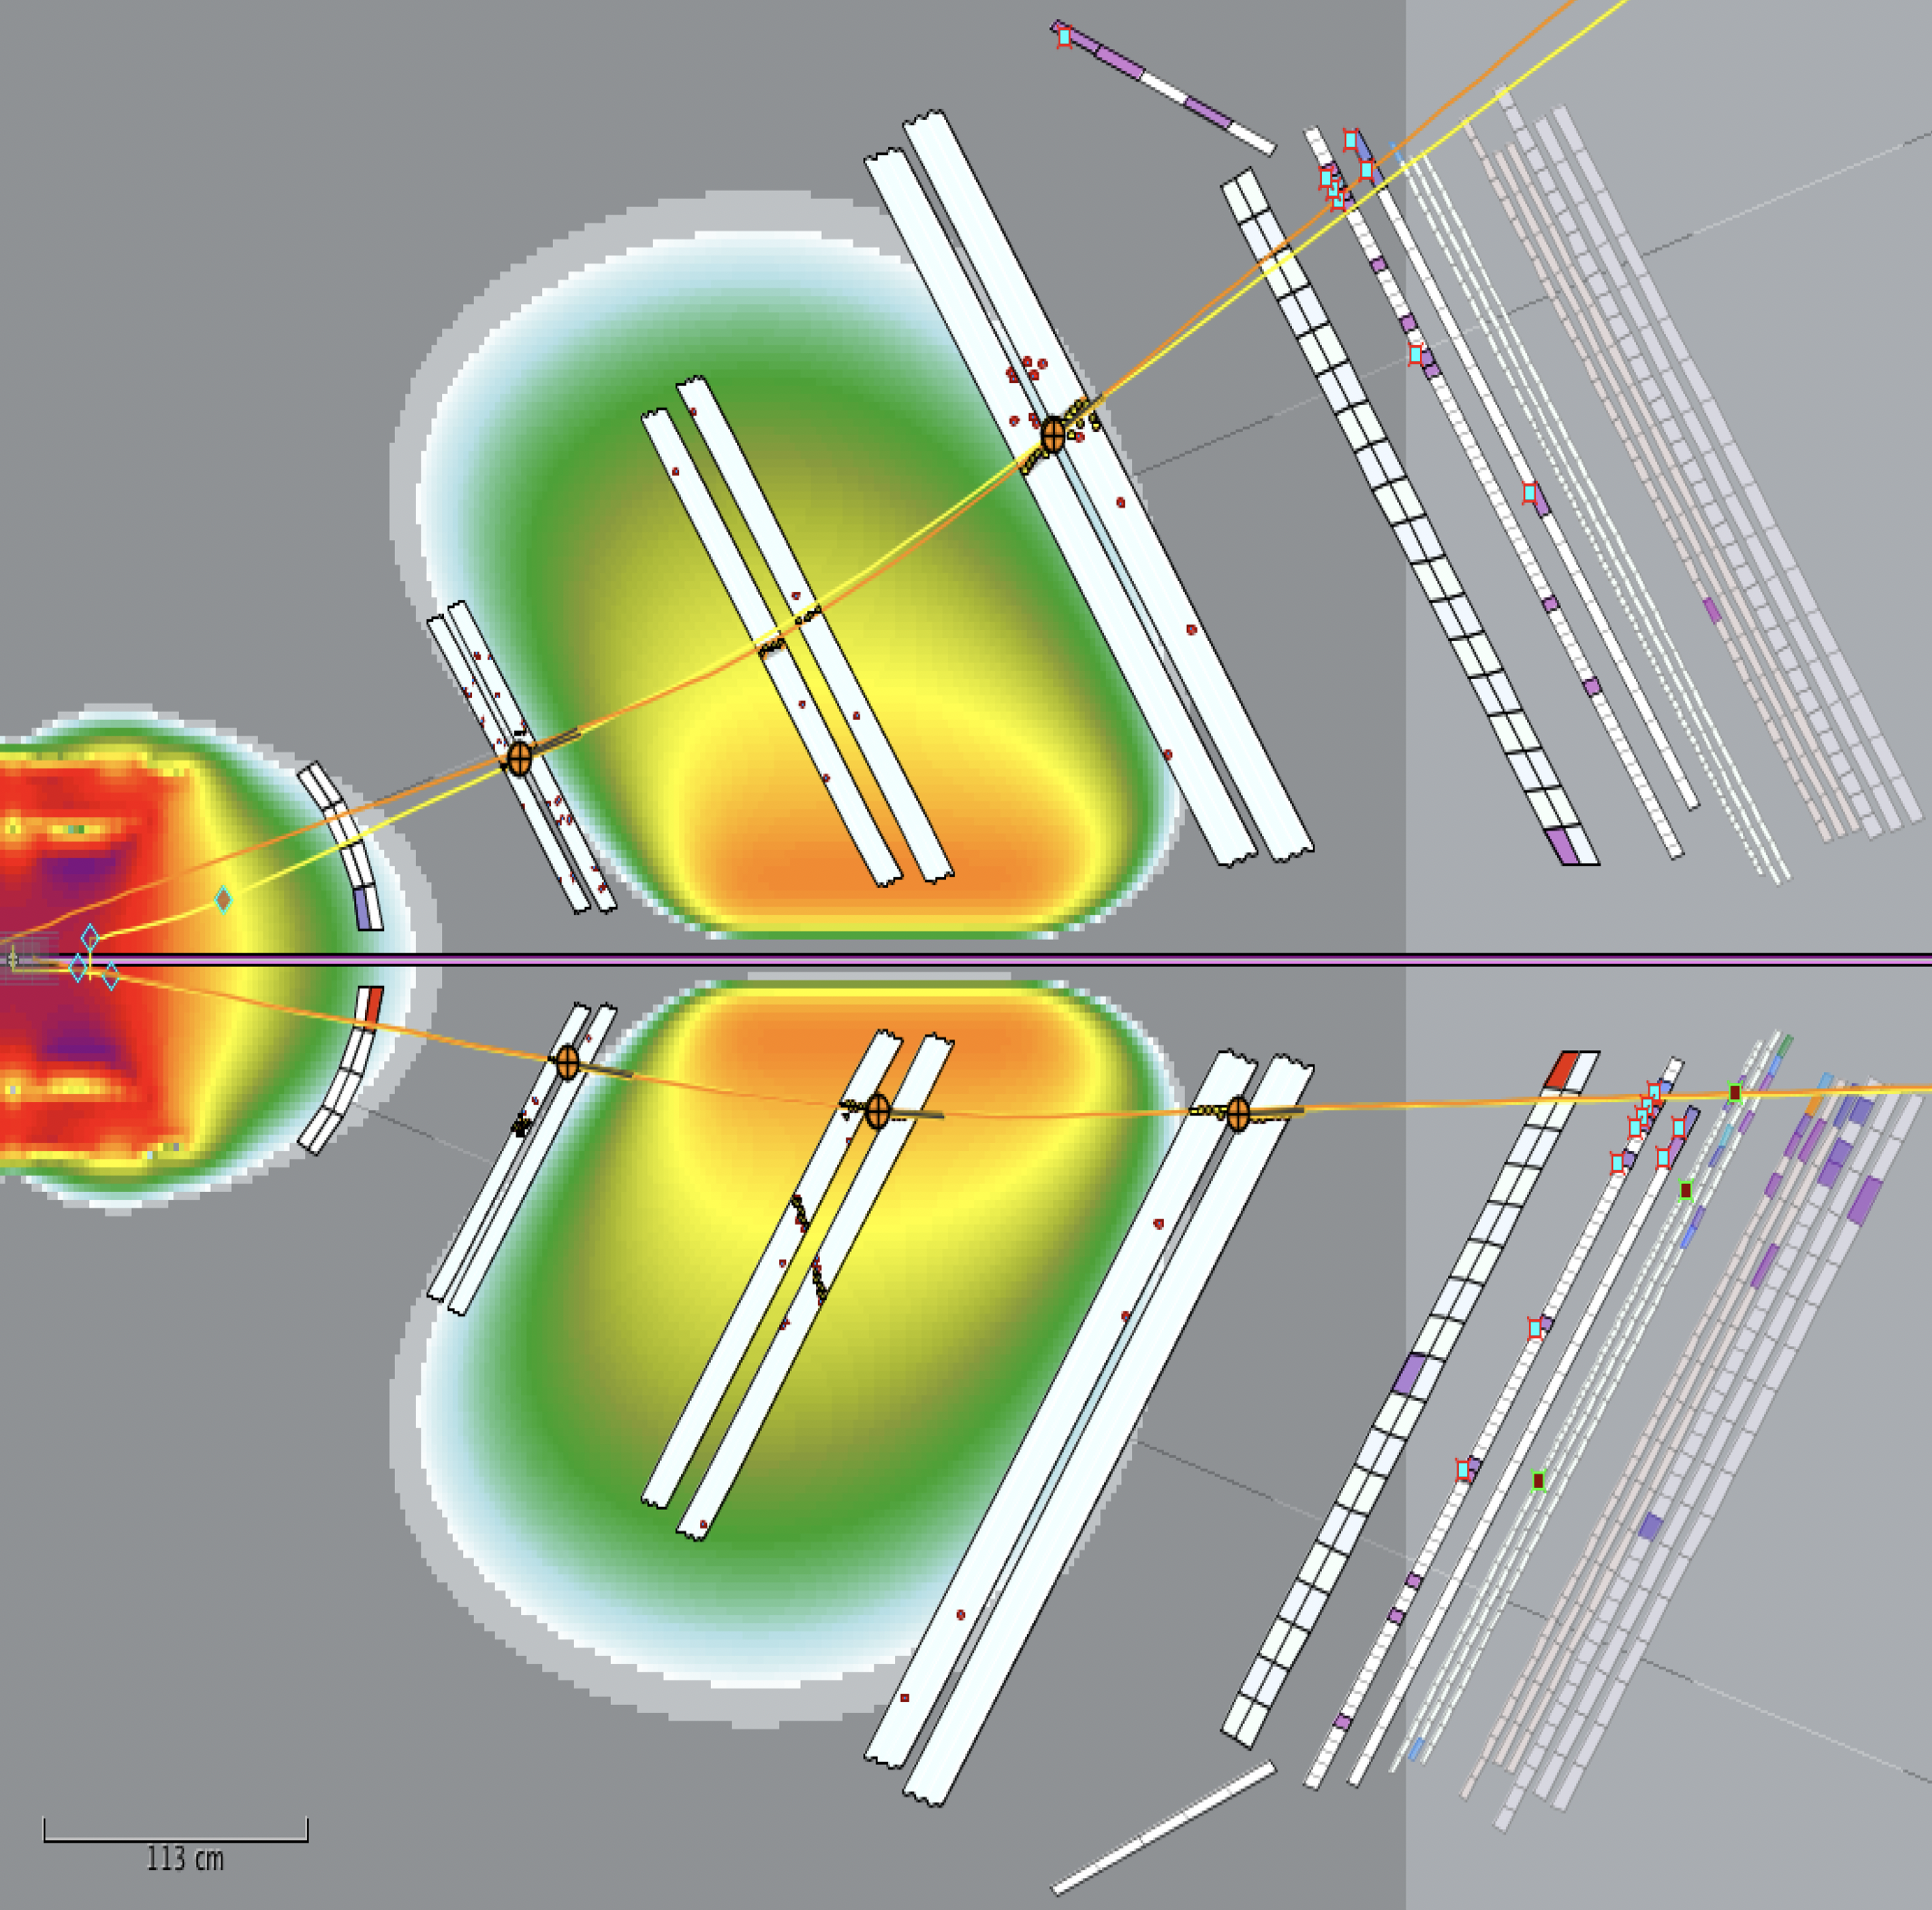
\includegraphics[width=1.0\columnwidth,keepaspectratio]{img/ced.png}
	\caption{CED Event Example}
	\label{fig:ced}
\end{figure}
